\documentclass[11pt]{article}
\usepackage{graphicx}
\DeclareGraphicsRule{.tif}{png}{.png}{`convert #1 `dirname #1`/`basename #1 .tif`.png}

\textwidth = 6.5 in
\textheight = 9 in
\oddsidemargin = 0.0 in
\evensidemargin = 0.0 in
\topmargin = 0.0 in
\headheight = 0.0 in
\headsep = 0.0 in
\parskip = 0.2in
\parindent = 0.0in
\usepackage{paralist} %compactenum

%\newtheorem{theorem}{Theorem}
%\newtheorem{corollary}[theorem]{Corollary}
%\newtheorem{definition}{Definition}
\usepackage{tipa}
\usepackage{amsfonts}
\usepackage[mathscr]{eucal}

% Use the natbib package for the bibliography
\usepackage[round]{natbib}
\bibliographystyle{apalike}
\newcommand{\exampleMacro}[1]{\mu_{#1}}

\renewcommand{\Pr}{{\mathbb P}}
\usepackage{wrapfig}
\usepackage{bm}
\usepackage{listings}
\usepackage{url}
\usepackage{algorithm}
\usepackage{algorithmic}
\usepackage{pgf}
\include{positioning}
\usepackage{tikz}
\usetikzlibrary{trees,arrows,positioning,scopes}
\tikzset{terminal/.style={rectangle,minimum size=6mm,rounded corners=3mm,very thick,draw=black!50, top color=white,bottom color=black!20, font=\ttfamily}}
\tikzset{hidden/.style={rectangle,draw=white,fill=white,thick}}
\tikzset{analysis/.style={rectangle,rounded corners,draw=black!50,fill=white,thick,minimum width=6cm}}
\tikzset{charmatrix/.style={rectangle,draw=none,fill=black,minimum width=6cm,minimum height=8mm}}
\tikzset{augmat/.style={rectangle,draw=none,fill=red,minimum width=6cm,minimum height=15mm}}
\tikzset{tree/.style={rectangle,draw=black,fill=black,minimum width=6cm,minimum height=8mm}}
\tikzset{inf/.style={rectangle,rounded corners,draw=black!50,fill=green!20,thick,minimum width=6cm,minimum height=2cm}}
\tikzset{toArrow/.style={stealth-,ultra thick}}


%\newcommand{\newAppendix}[2]{
%	\addtocounter{appendixCounter}{1}
%	{\bf Appendix {\arabic{appendixCounter}\label{#2}}: #1}
%	}


\usepackage{hyperref}
\hypersetup{backref,  pdfpagemode=FullScreen,  linkcolor=blue, citecolor=red, colorlinks=true, hyperindex=true}

\begin{document}
\newcounter{appendixCounter}

\section*{MCMC notes by Mark Holder}
\subsection*{Bayesian inference}
Ultimately, we want to make probability statements about true values of parameters, given our data. For example $\Pr(\alpha_0 < \alpha_1|X)$.
According to Bayes' theorem:
	$$\Pr(\theta|X) = \frac{\Pr(X|\theta)\Pr(\theta)}{\Pr(X)}$$
It is often the case that we cannot calculate $\Pr(X)$, the marginal probability of the data.


Markov chain Monte Carlo is (by far), the dominant computational approach to conducting Bayesian inference.
The ``Monte Carlo'' part of the name reflects the fact that we are going to perform a random simulation -- the algorithm uses a pseudo-random number generator to explore parameter space.
The ``Markov chain'' part of the name refers to fact that we are going to conduct the simulation by iteratively updating the state of the simulator using rules that depend only on the current state of the system.
This type of stochastic system (one which ``forgets'' its history) is referred to as a Markov chain.

\subsection*{Markov chains}
A Markov chain is a series of states.
You can think of it as a walk through a ``state space''.
\begin{compactitem}
	\item a {\em state} is the complete description of the ``value'' of the chain as it walks.  We'll be walking through parameter space, so the state space is the space of all parameter values in our model.
	Typically the state space is continuous, but I'll explain most of the theory in problems with discrete state space.
	\item an {\em index} refers to which step of the chain we are currently at. There are many uses for continuous-time Markov chains (in which the index can assume any numerical value), but the Markov chains that we will be using in MCMC are discrete time.  This means that the index is simply a count of the number iterations that the algorithm has been running.  The index is often referred to as the ``iteration,'' the ``generation,'' or the ``step number.''  In a discrete time Markov chain, you update the state once per interval (although you can remain in the same state and still consider that an update).
\end{compactitem}

There is a huge literature on Markov processes, but there are only a few crucial aspects of Markov chains that we need to understand if we want to understand MCMC.
\begin{compactitem}
	\item Under mild conditions, a Markov chain will converge to a stationary distribution (also called a steady-state distribution) after a large number of steps. This distribution will be the same regardless of the starting point of the chain.
	\item Markov chains that have a high probability of changing state in a single step will converge to the stationary distribution faster.
\end{compactitem}

\subsubsection*{Transition probabilities}
A Markov chain can be defined by describing the full set of probability statements that define the rules for the state of the chain in the next step (step $i+1$) given its current state (in step $i$).
These transition probabilities are analogous to transition rates if we are working with continuous-time Markov processes.

\begin{wrapfigure}{r}{5cm}
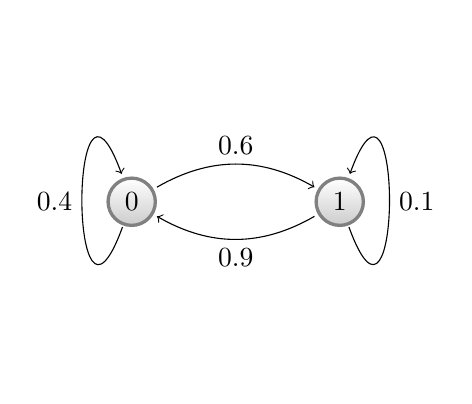
\begin{tikzpicture} 
  \node[terminal] (zero) {$0$};
  \node[terminal,right=2cm of zero] (one) {$1$};
  \draw[->] (zero) edge[bend left] node (f) [above]{0.6} (one)
  		    (zero) edge [out=250, in=110, looseness=1,distance=3cm, loop] node[left] {$0.4$} (zero)
            (one) edge[bend left] node (h) [below]{$0.9$} (zero)
            (one) edge [out=290, in=70, looseness=1,distance=2cm, loop] node[right] {$0.1$} (zero)
            ;
\end{tikzpicture}
\caption{A graphical depiction of a two-state Markov process.}\label{fig2state}
\end{wrapfigure}
Consider the simplest possible Markov chain: one with two states (0, and 1) that operates in discrete time.
The figure to the right shows the states in circles. 
The transition probabilities are shown as arcs connecting the states with the probabilities next to the line.
The full probability statements that correspond to the graph are:
\begin{eqnarray*}
	\Pr(x_{i+1}=0|x_i=0) & = & 0.4\\
	\Pr(x_{i+1}=1|x_i=0) & = & 0.6\\
	\Pr(x_{i+1}=0|x_i=1) & = & 0.9\\
	\Pr(x_{i+1}=1|x_i=1) & = & 0.1
\end{eqnarray*}
Note that, because these are probabilities, some of them must sum to one.
In particular, if we are in a particular state at step $i$ we can call the state $x_i$.  
In the next step, we must have {\em some} state so $1 = \sum_j \Pr(x_{i+1}=j|x_i)$ for every possible $x_i$.

Note that the state at step $i+1$ only depends on the state at step $i$. 
This is the Markov property. More formally we could state it as:
$$\Pr(x_{i+1}|x_i) = \Pr(x_{i+1}|x_i, x_{i-k}) $$
where $k$ is positive integer. 
What this probability statement is saying is that, conditional on $x_i$, the state at $i+1$ is independent on the state at any point before $i$.
So when working with Markov chains we don't need to concern ourselves with the full history of the chain, merely knowing the state at the previous step is enough.\footnote{There are second-order Markov processes that depend on the two previous states, and third-order Markov process {\em etc.}. But in this course, we'll just be dealing with the simplest Markov chains which only depend on the current state.}

Clearly if we know $x_i$ and the transition probabilities, then we can make a probabilistic statement about the state in the next iteration (in fact the transition probabilities {\em are} these probabilistic statements).
But we can also think about the probability that the chain will be in a particular state two steps form now:
\begin{eqnarray*}
	\Pr(x_{i+2}=0|x_i=0) & = & \Pr(x_{i+2}=0|x_{i+1}=1)\Pr(x_{i+1}=1|x_i=0) +  \Pr(x_{i+2}=0|x_{i+1}=0)\Pr(x_{i+1}=0|x_i=0)\\
					    & = & 0.9*0.6 +  0.4*0.4\\
					    & = & 0.7
\end{eqnarray*}
Here we are exploiting the fact that the same ``rules'' (transition probabilities) apply when we consider state changes between $i+1$ and $i+2$.
If the transition probabilities are fixed through the running of the Markov chain, then we are dealing with a time-homogeneous Markov chain.

Note that:
\begin{eqnarray*}
	\Pr(x_{i+2}=1|x_i=0) & = & \Pr(x_{i+2}=1|x_{i+1}=1)\Pr(x_{i+1}=1|x_i=0) +  \Pr(x_{i+2}=1|x_{i+1}=0)\Pr(x_{i+1}=0|x_i=0)\\
					    & = & 0.1*0.6 +  0.6*0.4\\
					    & = & 0.3
\end{eqnarray*}
So,  if we sum over all possible states at $i+2$, the relevant probability statements sum to one.

It gets tedious to continue this for a large number of steps into the future.
But we can ask a computer to calculate the probability of being in state $0$ for a large number of steps into the future by repeating the calculations (see the Appendix \ref{appendixCodeTwoProb} for code).
Figure (\ref{figProbTrace}) shows the probabilities of the Markov process being in state 0 as a function of the step number for the two possible starting states.

\begin{figure}[h]
\begin{picture}(0,230)(0,-100)
	\put(-30,20){\makebox(0,0)[l]{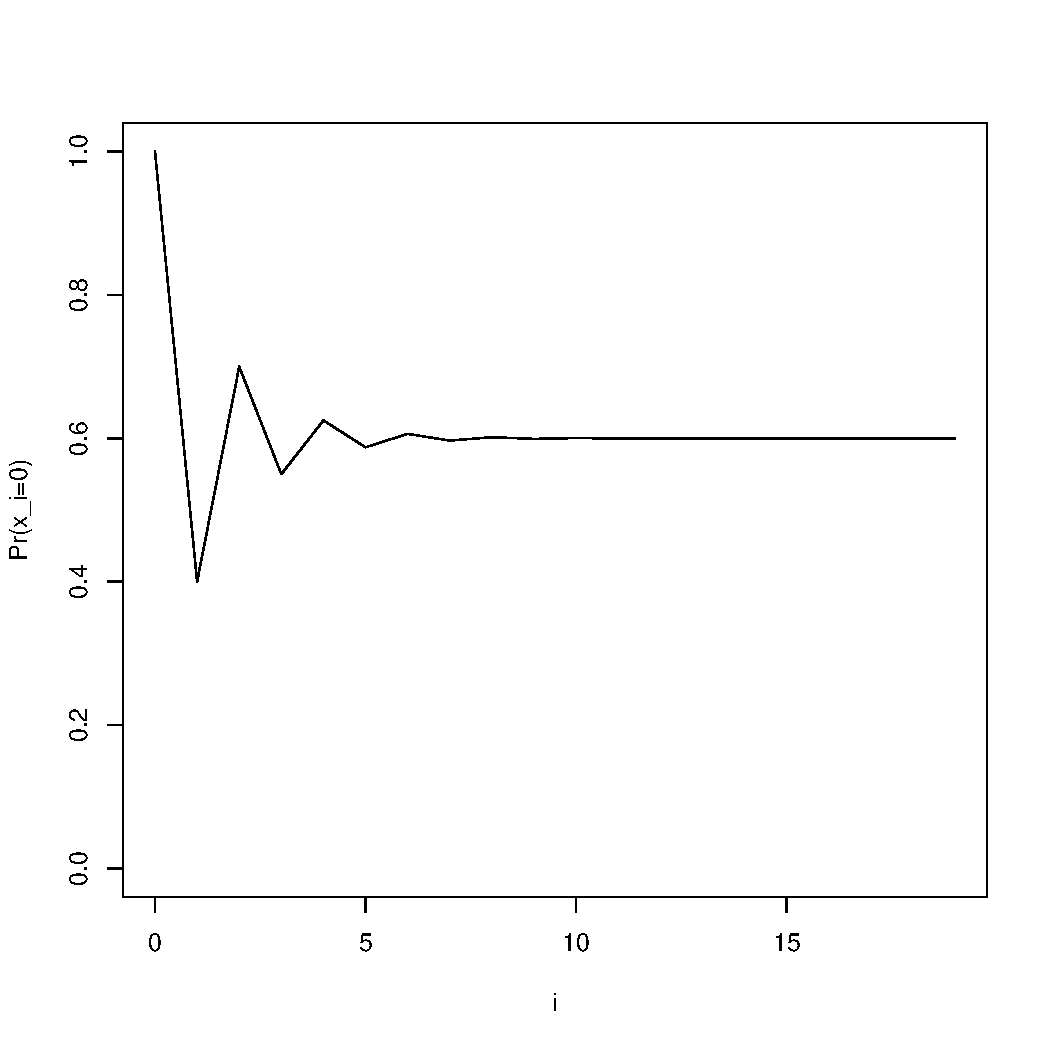
\includegraphics[scale=0.5]{start_from_0.pdf}}}
	\put(220,20){\makebox(0,0)[l]{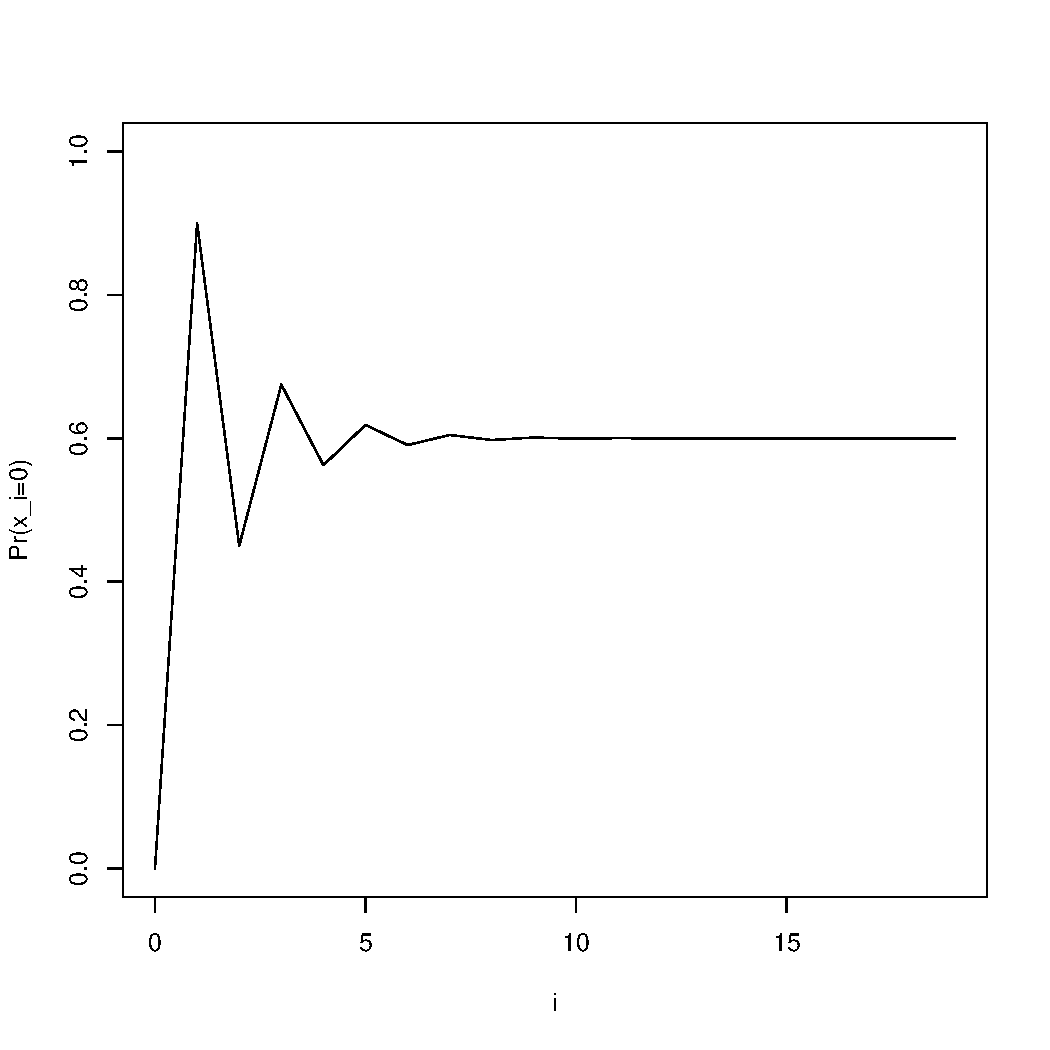
\includegraphics[scale=0.5]{start_from_1.pdf}}}
	\put(50,-105){\small $\Pr(x_i=0|x_0=0)$}
	\put(310,-105){\small $\Pr(x_i=0|x_0=1)$}
\end{picture}
\caption{The probability of being in state 0 as a function of the step number, $i$, for two different starting states (0 and 1) for the Markov process depicted in Figure (\ref{fig2state}).}\label{figProbTrace}
\end{figure}

Note that the probability stabilizes to a steady state distribution.
Knowing whether the chain started in state 0 or 1 tells you very little about the state of the chain in step 15.
Technically, $x_{15}$ and $x_0$ are {\em not} independent of each other.
If you work through the math the probability of the state at step 15 does depend on the starting state:
\begin{eqnarray*}
	\Pr(x_{15} = 0 | x_0 = 0) & = & 0.599987792969\\
	\Pr(x_{15} = 0 | x_0 = 1) & = & 0.600018310547
\end{eqnarray*}
But clearly the probabilities are very close.

If we consider an even large number of iterations (e.g. the state at step 100), then the probabilities are so close that they are indistinguishable.

After a long enough walk, a Markov chain in which all of the states are connected\footnote{The fancy jargon is ``irreducible.'' A reducible chain has some states that are disconnected from others, so the chain can be broken up (reduced) into two or more chains that operate on a subset of the states.} will {\em converge} to its stationary distribution.

\subsubsection*{Many chains or one really long chain}
When constructing arguments about Markov chains we often flip back and forth between thinking about the behavior of an arbitrarily large number of instances of the random process all obeying the same rules (but performing their walks independently) versus the behavior we expect if we sparsely sample a very long chain.
The idea is that if sample sparsely enough, the sampled points from one chain are close to being independent of each other (as Figure \ref{figProbTrace} was meant to demonstrate).
Thus we can think of a very long chain as if we had a large number of independent chains.


\subsubsection*{Stationary distribution}
Notice in the discussion above that the probability of ending up in state 0 as the number of iterations increased approached 0.6. What is special about this value?

It turns out that in the stationary distribution (frequently denoted $\bm \pi$), the probability of sampling a chain in state 0 is 0.6.
We would write this as $\bm \pi = \{0.6, 0.4\}$  or the pair of statements: $\bm \pi_0 = 0.6, \bm \pi_1 = 0.4$.

How can we show that this is the steady-state (equilibrium) distribution?
The flux ``out'' of each state must be equal to the ``flux'' into that state for a system to be at equilibrium.
Here it is helpful to think about running infinitely many chains.
If we have an equilibrium probability distribution, then we can characterize the probability of a chain leaving state 0 in at one particular step in the process.
This is the joint probability of being in state 0 at step $i$ and the probability of an $0 \rightarrow 1 $ transition at point $i$.
Thus,
\begin{eqnarray*}
	\Pr(0 \rightarrow 1 \mbox{ at } i) & = & \Pr(x_i = 0)\Pr(x_{i+1} = 1| x_i = 0)
\end{eqnarray*}
At the equilibrium $ \Pr(x_i = 0) = \bm \pi_0$, so the flux out of 0 at step $i$ is $\bm \pi_0 \Pr(x_{i+1} = 1| x_i = 0)$.
In our simple (two-state) system the flux into state 0 can only come from state 1, so:
\begin{eqnarray*}
	\Pr(1 \rightarrow 0 \mbox{ at } i) & = & \Pr(x_i = 1)\Pr(x_{i+1} = 0| x_i = 1) \\
		& = & \bm \pi_1\Pr(x_{i+1} = 0| x_i = 1) 
\end{eqnarray*}
If we force the ``flux out'' and ``flux in'' to be identical:
\begin{eqnarray*}
	\bm \pi_0 \Pr(x_{i+1} = 1| x_i = 0) & = & \bm \pi_1\Pr(x_{i+1} = 0| x_i = 1) \\
	\frac{\bm \pi_0}{\bm \pi_1} & = & \frac{\Pr(x_{i+1} = 0| x_i = 1)}{\Pr(x_{i+1} = 1| x_i = 0)} 
\end{eqnarray*}
We can then solve for the actual frequencies by recognizing that $\bm \pi$ is a probability distribution:
\begin{eqnarray*}
	\sum_k \bm \pi_k & = & 1
\end{eqnarray*}
For the system that we are considering:
\begin{eqnarray*}
	\frac{\bm \pi_0}{\bm \pi_1} & = & \frac{0.9}{0.6} = 1.5  \\
	\bm \pi_0 & = & 1.5\bm \pi_1 \\
	1.5\bm \pi_1 + \bm \pi_1 & = & 1.0 \\
	\bm \pi_1 & = & 0.4 \\
	\bm \pi_0 & = &  0.6
\end{eqnarray*}

Thus, the transition probabilities determine the stationary distribution.

{\bf If we can choose the transition probabilities then we can construct a sampler that will converge to any distribution that we would like.}

When we have a state set $\mathcal{S}$ with more than 2 states, we can express a general statement about the stationary distribution:
\begin{equation}
	\bm\pi_j = \sum_{k\in \mathcal{S}}\bm\pi_{k}\Pr(x_{i+1} = j|x_{i} = k) \label{generalEquil}
\end{equation}
The connection to the ``flux out'' and ``flux in'' argument may not seem obvious, but note that the ``flux out'' can be 
quantified in terms of the 1 - the ``self-transition.''
Let $\mathcal{S}_{\neq j}$ be the set of states that excludes state $j$, so the ``flux out'' is:
\begin{eqnarray*}
	\mbox{flux out of } j & = & \bm\pi_j\Pr(x_{i+1}\in\mathcal{S}_{\neq j}|x_i=j) \\
	 & = &  \bm\pi_j\left[1 - \Pr(x_{i+1}\in j|x_i=j)\right]\\
\end{eqnarray*}
The flux in is:
\begin{eqnarray*}
	\mbox{flux into } j & = & \sum_{k\in \mathcal{S}_{\neq j}}\pi_{k}\Pr(x_{i+1} = j|x_{i} = k) \\
\end{eqnarray*}
Forcing the fluxes to be equal gives us:
\begin{eqnarray}
	\bm\pi_j\left[1 - \Pr(x_{i+1} =  j|x_i=j)\right] & = & \sum_{k\in \mathcal{S}_{\neq j}}\bm\pi_{k}\Pr(x_{i+1} = j|x_{i} = k) \nonumber \\
	\bm\pi_j & = &  \bm\pi_j\Pr(x_{i+1} =  j|x_i=j) + \sum_{k\in\mathcal{S}_{\neq j}}\bm \pi_{k}\Pr(x_{i+1} = j|x_{i} = k)    \label{separatedGenEq} \\
	& = & \sum_{k\in\mathcal{S}}\bm \pi_{k}\Pr(x_{i+1} = j|x_{i} = k) \nonumber
\end{eqnarray}



\subsubsection*{Mixing}
We just saw how changing transition probabilities will affect the stationary distribution. 
Perhaps, there is a one-to-one mapping between transition probabilities and a stationary distribution.
In the form of a question: if we were given the stationary distribution could we decide what the transition rates must be to achieve that distribution?

It turns out that the answer is ``No.''  
Which can be seen if we examine equation (\ref{separatedGenEq}).
Imagine dropping the flux out of each state by a factor of 10.
Because the ``self-transition'' rate would increase by the appropriate amount, we can still end up in the same stationary distribution.

How would such a chain behave? The primary difference is that it would ``mix'' more slowly.
Adjacent steps would be more likely to be in the same state, and it would take a larger number of iterations before the chain ``forgets'' its starting state.
Figure (\ref{figProbTraceSlow}) depicts the same probability statements as Figure (\ref{figProbTrace}) but for a process in which $\Pr(x_{i+1}=1|x_i=0) = 0.6 $ and $\Pr(x_{i+1}=0|x_i=1) = 0.9$.
\begin{figure}[h]
\begin{picture}(0,230)(0,-100)
	\put(-30,20){\makebox(0,0)[l]{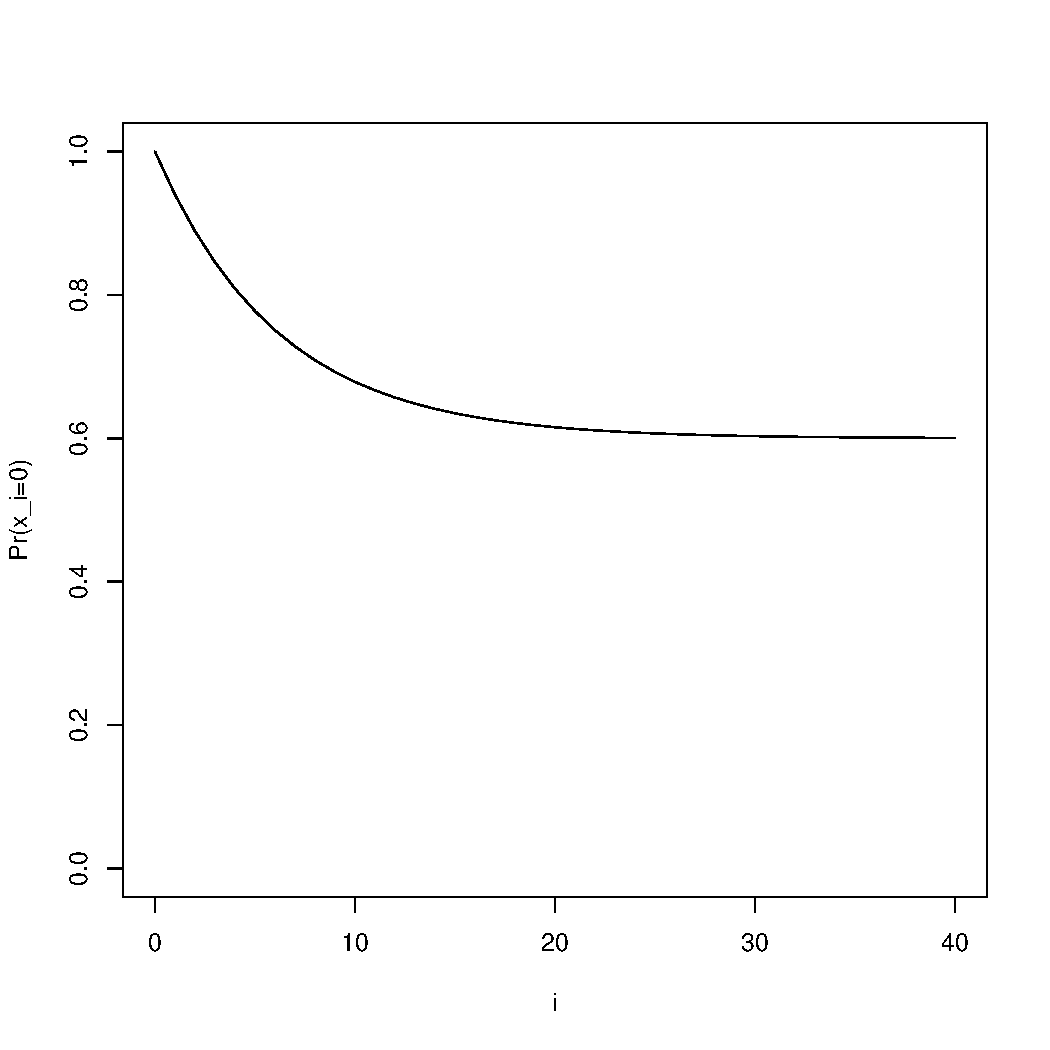
\includegraphics[scale=0.5]{start_from_0_slow.pdf}}}
	\put(220,20){\makebox(0,0)[l]{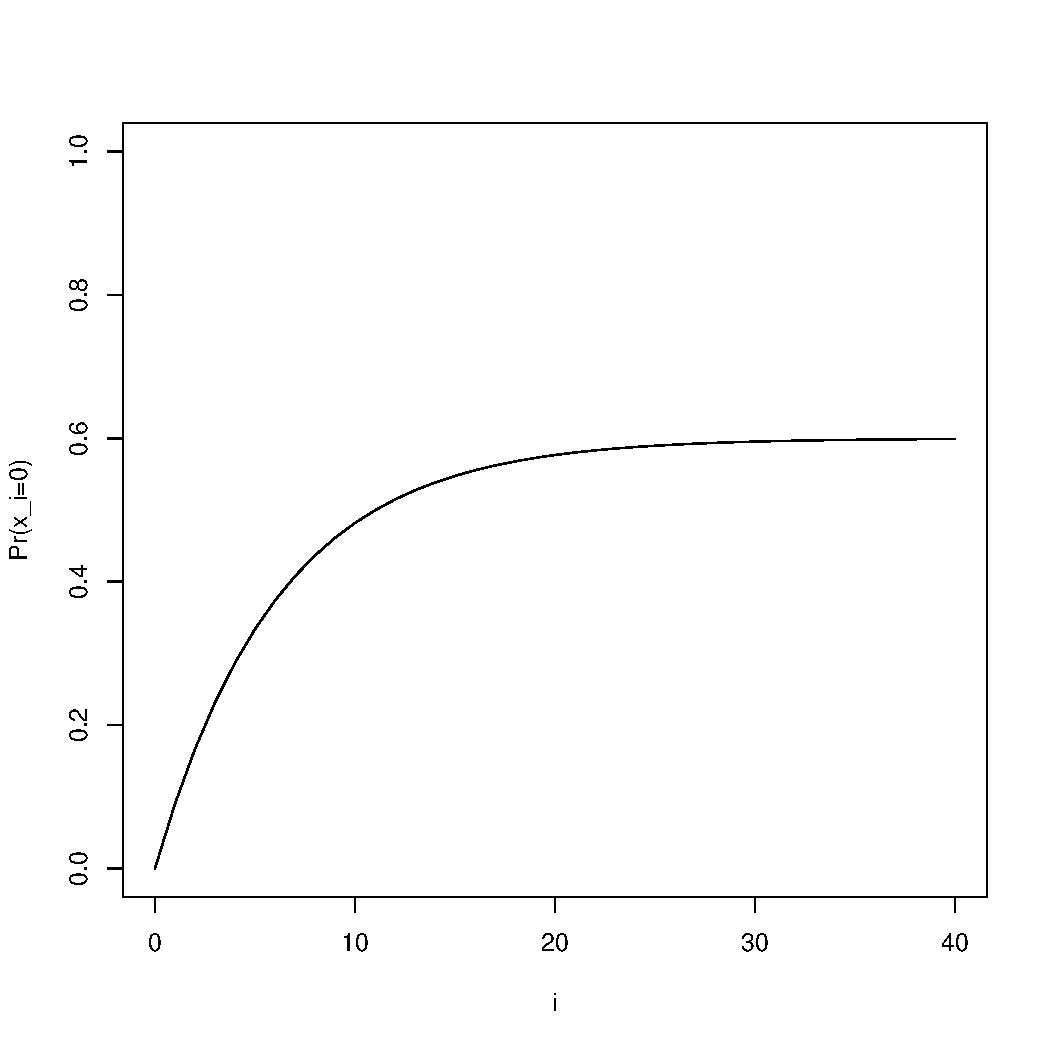
\includegraphics[scale=0.5]{start_from_1_slow.pdf}}}
	\put(50,-105){\small $\Pr(x_i=0|x_0=0)$}
	\put(310,-105){\small $\Pr(x_i=0|x_0=1)$}
\end{picture}
\caption{The probability of being in state 0 as a function of the step number, $i$, for two different starting states (0 and 1) for the Markov process depicted in Figure (\ref{fig2state}) but with the state-changing transition probabilities scaled down by a factor of 10.  Compare this to Figure (\ref{figProbTrace}).}\label{figProbTraceSlow}
\end{figure}

Thus, that the rate of convergence of a chain to its stationary distribution is an aspect of a Markov chain that is separate from what the stationary distribution is.

In MCMC we will design a Markov chain such that its stationary distribution will be identical to the posterior probability distribution over the space of parameters.
We will try to design chains that have high transition probabilities, so that our MCMC approximation will quickly converge to the posterior.
But even a slowly mixing chain will (in theory) eventually be capable of providing an approximation to the posterior probability.


\subsection*{Detailed Balance}
In principle, we could use the information in Equation (\ref{generalEquil}) to inform us as to how to construct a chain with a desired $\bm \pi$.
In practice, this is difficult when we have a large number of states.
In the continuous parameter case, we have an infinite number of states and the summation becomes an integral.

Setting transition probabilities in a general way such that the total flux into and out of any state satisfies the property shown in Equation (\ref{generalEquil}) is tricky.

Typically, we restrict ourselves to a subset of possible Markov chains: those that satisfy detailed balance for all pairs of states $j$ and $k$:
\begin{eqnarray}
	\bm \pi_j\Pr(x_{i+1} = k| x_i = j) = \bm \pi_k\Pr(x_{i+1} = j| x_i = k) \label{theDeets}
\end{eqnarray}
Detailed balance means that for any two possible states, the flux between them balances out.

Clearly, if the flux out of $j$ into $k$ is exactly matched by the flux from $k$ into $j$, then  Equation (\ref{generalEquil}) will also be satisfied (the total flux out of $j$ will be balanced by the total flux into $j$).

\section*{MCMC}
In the Metropolis-Hastings algorithm, we choose rules for constructing a stochastic walk through parameter space.
We adopt transition probabilities such that the stationary distribution of our Markov chain is equal to posterior probability distribution.
In notation we would like:
$$ \bm \pi_{\theta_j} = \Pr(\theta_j|\mbox{Data})$$

Let's work through an example for which we can calculated the posterior probabilities analytically, and then construct a MCMC algorithm that will converge to those posterior probabilities.

\subsection*{Double-headed coin}
Imagine a store that sells four-packs of quarters, but in some of the packs some of the coins have George Washington's head on both sides ($\Pr(H) = 1$ for these coins) while the remaining coins are fair coins ($\Pr(H)  = \Pr(T)  = 0.5$).

Further more there are equal numbers of packages that contain 0, 1, 2, 3, or 4 double-headed coins, and the packages are not labelled.

Someone grabs a package at random and records the number of heads from two experiments in which all for coins are flipped.
In the first experiment all four flips are heads.
In the second experiment three of the four flips are heads.

We want to make a probability statement about the number of coins in the pack that are double-headed.
Thus our data is $D=\{d_1=4, d_2=3\}$.
We have one parameter, $\theta$, which can take on 5 values: $\theta\in\{0,1,2,3,4\}$. 

If the five times of packs are equally likely, then we can express the prior probability of each value of $\theta$ as $1/5$.

We can calculate the probability of different number of heads, $h$, given each possible value of $\theta$ by calculating the probability of $h-\theta$ heads in $4-\theta$ flips.
We use these likelihood calculations and Bayes formula:
$$ \Pr(\theta|D) = \frac{\Pr(D|\theta)\Pr(\theta)}{\Pr(D)}= \frac{\Pr(D,\theta)}{\Pr(D)}$$ 
to produce the following table:
\begin{table}[htdp]
\begin{center}
\begin{tabular}{|c|c|c|c|c|c|c|}
\hline
& \multicolumn{5}{c|}{$\theta$} &\\
& 0 & 1 & 2 & 3 & 4 & Sum\\
\hline
$\Pr(d=4|\theta)$ & 1/16 & 2/16 & 4/16 & 8/16 & 16/16 & \\
$\Pr(d=3|\theta)$ & 4/16 & 6/16 & 8/16 & 8/16 & 0 & \\
$\Pr(d=2|\theta)$ & 6/16 & 6/16 & 4/16 & 0 & 0 & \\
$\Pr(d=1|\theta)$ & 4/16 & 2/16 & 0 & 0 & 0 & \\
$\Pr(d=0|\theta)$ & 1/16 & 0 & 0 & 0 & 0 & \\
\hline
$\sum_{i=0}^4 \Pr(d=i|\theta)$ & 1 & 1 & 1 & 1 & 1 & \\
\hline
$\Pr(d_1=4|\theta)$ & 1/16 & 2/16 & 4/16 & 8/16 & 16/16 & \\
$\Pr(d_2=3|\theta)$ & 4/16 & 6/16 & 8/16 & 8/16 & 0 & \\
$\Pr(D|\theta)$  & 4/256 & 12/256 & 32/26 & 64/256 & 0 & \\
\hline
$\Pr(\theta)$ & 0.2 & 0.2 & 0.2 & 0.2 & 0.2 & 1\\ 
\hline
$\Pr(\theta,D)$  & 4/1280 & 12/1280 & 32/1280 & 64/1280 & 0 & \\
$\Pr(D) =\sum_{\theta}\Pr(\theta,D)$ & & & & & & 112/1280 \\
\hline
$\Pr(\theta|D) = \frac{\Pr(D,\theta)}{\Pr(D)}$ & 1/28 & 3/28 & 2/7 & 4/7 & 0 & 1\\
\hline
\end{tabular}
\end{center}
\label{default}
\end{table}

\subsection*{MCMC}
In this case, we can simply calculate the posterior probability of $\theta$ given the data.  
But, in more complicated scenarios we cannot perform calculations for all possible values of $\theta$.
When we cannot try all possible values of $\theta$, then we can't sum them to get $\Pr(D)$.
In fact, our inability to calculate $\Pr(D)$, the marginal probability of the data, is the primary reason that we usually have to resort to MCMC to perform Bayesian inference.

Recall, that in MCMC we are going to explore the space of parameters.  
In the case of the coin-example, there are 5 possible values for $\theta$.
So we need to construct a Markov chain with 5 states.
\begin{figure}
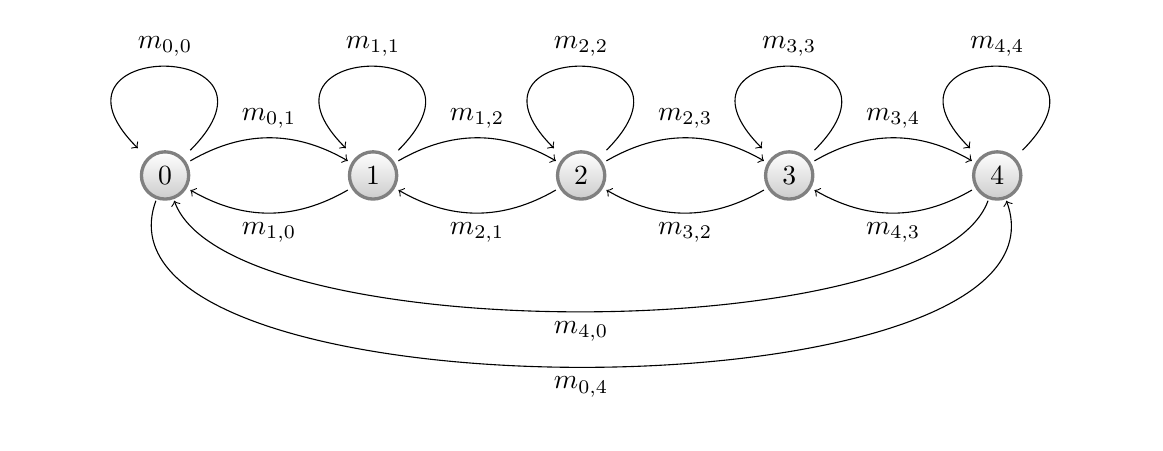
\begin{tikzpicture} 
  \node[terminal] (zero) {$0$};
  \node[terminal,right=2cm of zero] (one) {$1$};
  \node[terminal,right=2cm of one] (two) {$2$};
  \node[terminal,right=2cm of two] (three) {$3$};
  \node[terminal,right=2cm of three] (four) {$4$};
  \draw[->] (zero) edge[bend left] node (f) [above]{$m_{0,1}$} (one)
  		    (one) edge[bend left] node (f) [above]{$m_{1,2}$} (two)
  		    (two) edge[bend left] node (f) [above]{$m_{2,3}$} (three)
  		    (three) edge[bend left] node (f) [above]{$m_{3,4}$} (four)
  		    (zero) edge [loop] node[above] {$m_{0,0}$} (zero)
  		    (one) edge [loop] node[above] {$m_{1,1}$} (one)
  		    (two) edge [loop] node[above] {$m_{2,2}$} (one)
  		    (three) edge [loop] node[above] {$m_{3,3}$} (one)
  		    (four) edge [loop] node[above] {$m_{4,4}$} (one)
            (four) edge[out=250, in=290, looseness=1,distance=2cm] node (h) [below]{$m_{4,0}$} (zero)
            (zero) edge[out=250, in=290, looseness=.5,distance=3cm] node (h) [below]{$m_{0,4}$} (four)
            (one) edge[bend left] node (h) [below]{$m_{1,0}$} (zero)
            (two) edge[bend left] node (h) [below]{$m_{2,1}$} (one)
            (three) edge[bend left] node (h) [below]{$m_{3,2}$} (two)
            (four) edge[bend left] node (h) [below]{$m_{4,3}$} (three)
            ;
\end{tikzpicture}
\caption{A graphical depiction of a five-state Markov process.}\label{fig5state}
\end{figure}



\subsection*{GLM in Bayesian world}
Consider a data set of different diets many full sibs reared under two diets (normal=0, and unlimited=1).
We measure snout-vent length for a bunch of gekkos.
Our model is:
\begin{compactitem}
	\item There is an unknown mean SVL under the normal diet, $\alpha_0$.
	\item $\alpha_1$ is the mean SVL of an infinitely-large independent sample under the unlimited diet.
	\item Each family, $j$, will have a mean effect, $B_j$. This effect gets added to the mean based on the diet, regardless of diet.
	\item Each family, $j$, will have a mean response to unlimited diet, $C_{1j}$. This effect is only added to individuals on the unlimited diet. For notational convenience, we can simply define $C_{0j}=0$ for all families.
	\item The SVL for each individual is expected to normally-distributed around the expected value; the difference between a response and the expected value is $\epsilon_{ijk}$.
\end{compactitem}
To complete the likelihood model, we have to say something about the probability distributions that govern the random effects:
\begin{compactitem}
	\item $B_j \sim \mathcal{N}(0, \sigma_B)$
	\item $C_{1j} \sim \mathcal{N}(0, \sigma_C)$
	\item $\epsilon_{ijk} \sim \mathcal{N}(0, \sigma_E)$
\end{compactitem}

In our previous approach, we could do a hypothesis test such as $H_0: \alpha_0 = \alpha_1$, or we could generate point estimates.
That is OK, but what if we want to answer questions such as ``What is the probability that $\alpha_1 - \alpha_0 > 0.5$mm?''

Could we:
\begin{compactitem}
	\item reparameterize to $\delta_1 = \alpha_1 - \alpha_1$,
	\item construct a $x\%$ confidence interval,
	\item search for the largest value of $x^{\dag}$ such that 0 is not included in the confidence interval?
	\item do something like $\Pr(\alpha_1 - \alpha_0 > 0.5) = (1-x^{\dag})/2$
\end{compactitem}
, or something like that? {\bf No!} That is not a correct interpretation of a $P$-value, or confidence interval!

\newpage

\appendix
\section{Code to calculate probabilities for two-state Markov chain}\label{appendixCodeTwoProb}
Python code, {\tt two\_state.py}, to generate probabilities for a certain number of iterations:
\begin{lstlisting}[frame=single,language=Python,columns=fixed,upquote=false,showstringspaces=false]
#!/usr/bin/env python
import sys
from random import random as uniform

a_to_b = float(sys.argv[1])
assert(a_to_b > 0.0 and a_to_b <= 1.0)
b_to_a = float(sys.argv[2])
assert(b_to_a > 0.0 and b_to_a <= 1.0)
ti_prob_list = [a_to_b, b_to_a]
b_to_b = 1 - b_to_a
state = int(sys.argv[4])
assert(state in [0,1])
if state == 0:
    prob_list = [1.0, 0.0]
else:
    prob_list = [0.0, 1.0]
num_it = int(sys.argv[3])
assert(num_it > 0)

print "Gen\tPrZero\tPrOne"
for i in xrange(num_it):
    print "\t".join([str(i)] + [str(p) for p in prob_list])
    pb = prob_list[0]*a_to_b + prob_list[1]*b_to_b
    prob_list = [1-pb, pb]
\end{lstlisting}
R code, {\tt plotProbTrace.R}, to create plots from a file with columns labelled ``Gen'' and ``PrZero'':
\begin{lstlisting}[frame=single,language=S,columns=fixed,upquote=false,showstringspaces=false]
fn = commandArgs(TRUE)
d = read.table(fn, header=TRUE, sep="\t");
pdf(paste(fn, '.pdf', sep=""));
plot(d$Gen, d$PrZero, xlab="i", ylab="Pr(x_i=0)", type="l", ylim=c(0,1));
dev.off();
\end{lstlisting}
bash invocation using the scripts to create pdf documents:
\begin{lstlisting}[frame=single,language=bash,columns=fixed,upquote=false,showstringspaces=false]
$ python two_state.py 0.6 0.9 20 0 >start_from_0.txt
$ R --no-save -f plotProbTrace.R --args start_from_0.txt
$ python two_state.py 0.6 0.9 20 1 >start_from_1.txt
$ R --no-save -f plotProbTrace.R --args start_from_1.txt
\end{lstlisting}

\bibliography{phylo}
\end{document}  
